% Sections removed from the paper version of the document
% are marked with
% XXXX  Removed from paper version

\documentclass[a4paper]{article}
\usepackage[latin1]{inputenc}
\usepackage[left=4.4cm,top=3.05cm, right=4.5cm]{geometry}
\usepackage{xspace}
\usepackage{setspace}
\usepackage{courier}
\usepackage{hyperref}
\hypersetup{
    hidelinks,
    pdffitwindow=false,     % window fit to page when opened
    pdfstartview={FitH},    % fits the width of the page to the window
    pdftitle={RADDOSE-3D Command Reference},    % title
    pdfauthor={Zeldin, O. B.; Gerstel, M.; Garman, E. F.},     % author
   % pdfsubject={},   % subject of the document
    pdfcreator={Gerstel, M.},   % creator of the document
}
\RequirePackage{graphicx}
\usepackage{textcomp}

%%%%%%%%%%%%%%%%%%%%%%%%%%%%%%%%%%%%%%%%%%%%%%%%%%%%%%%%%%%%%%
%
%  temporary margin adjustment

\usepackage{chngpage}

% \begin{adjustwidth}{-1in}{-1in}% adjust the L and R margins by 1 inch
%  ..
% \end{adjustwidth}
%
%%%%%%%%%%%%%%%%%%%%%%%%%%%%%%%%%%%%%%%%%%%%%%%%%%%%%%%%%%%%%%


\usepackage[absolute,overlay]{textpos}
\setlength{\TPHorizModule}{1cm}
\setlength{\TPVertModule}{\TPHorizModule}
\textblockorigin{0mm}{20mm} % start everything near the top-left corner

\newcommand{\RD}{\texttt{RADDOSE-3D}\xspace}
\newcommand{\Class}[1]{\texttt{#1}\xspace}
\newcommand{\Function}[1]{\textit{#1}\xspace}
\newcommand{\Keyword}[1]{\texttt{\textbf{#1}}\xspace}
\newcommand{\SB}{\\[0.2em]}
\newcommand{\RDLegacyKeyword}{This keyword only has an effect when the absorption and attenuation coefficients are estimated using a legacy version of RADDOSE (see \hyperref[abscoefcalc]{section \ref*{abscoefcalc}}).\SB
}

\begin{document}
%\addtolength{\voffset}{-1in}
%\addtolength{\textheight}{1in}
\begin{center}
\noindent \textsf{\huge\textbf{\RD Command Reference}}\\[0.3em]
Dated: 1 May 2018\\[3.5em]
\end{center}

\noindent
Please cite the following primary publication when using \RD:\\[0.4em]
\href{http://dx.doi.org/10.1107/S0021889813011461}{\large\textbf{\RD: time- and space-resolved modelling\\[0.0em] of dose in macromolecular crystallography}}\\[0.1em]
\href{http://dx.doi.org/10.1107/S0021889813011461}{Zeldin, O. B.; Gerstel, M. \& Garman, E. F. (2013). \textit{J. Appl. Cryst.} \textbf{46} %, ??--??
}\\[0.1em]
\href{http://dx.doi.org/10.1107/S0021889813011461}{doi:10.1107/S0021889813011461}
\\[1.5em]
\noindent
For dose calculations related to SAXS experiments, please cite:\\[0.4em]
\href{https://doi.org/10.1107/S1600577516015083}{\large\textbf{Development of tools to automate quantitative analysis of radiation damage in SAXS experiments}}\\[0.1em]
\href{https://doi.org/10.1107/S1600577516015083}{Brooks-Bartlett, J. C.; Batters, R. A.; Bury, C. S.; Lowe, E. D.; Ginn, H. M.; Round, A., \& Garman, E. F. (2017). \textit{J. Synch. Rad.} \textbf{24} %, ??--??
}\\[0.1em]
\href{https://doi.org/10.1107/S1600577516015083}{doi:10.1107/S1600577516015083}
\\[1.5em]
\noindent
For more recent developments in \RD, including the ability to incorporate experimental profiles and irregular polyhedral crystal geometries, as well as the inclusion of  models for energy loss from the crystal volume due to the Compton effect and photoelectron escape, please additionally refer to:\\[0.4em]
\href{https://doi.org/10.1002/pro.3302}{\large\textbf{Estimate your dose: \RD}}\\[0.1em]
\href{https://doi.org/10.1002/pro.3302}{Bury, C. S.; Brooks-Bartlett, J. C.; Walsh, S. P. \& Garman, E. F. (2018). \textit{Protein Science} \textbf{27} %, ??--??
}\\[0.1em]
\href{https://doi.org/10.1002/pro.3302}{doi:10.1002/pro.3302}
\\[1.5em]

\tableofcontents

%\doublespacing
%\setstretch{3}

\newpage

\RD can take input from one or more files and/or from standard input (STDIN).
% XXXX  Removed from paper version
% in the final documentation instead of '.' continue with:
% using the \texttt{-i} command line parameter (see section \ref{commandline-input} of the supplementary material).
%When using this parameter a
Any input will be processed by the \Class{InputParser} class and the \RD ANTLR parser.
This section describes the syntax of accepted input.
Advanced users of \RD can create their own input method that need not rely on the \Class{InputParser} class or the \RD ANTLR parser. This feature will not be covered in this reference.

The simplest use case of \RD will involve only one file describing the entire experiment.
In some instances it may be desired to split up the input into a number of files, e.g. one file describing the crystal, one automatically updated file describing the current beam on the beamline, and one file chosen from a set of possible wedge strategies.
Each file can contain an arbitrary number (including none) of \Class{Crystal}, \Class{Beam} and \Class{Wedge} block (henceforth called \textit{blocks}). However, splitting up blocks across multiple files is not allowed.

The parser will read the input sequentially, and, when multiple sources are given, one source after the other in the specified order. While the parser may accept \Class{Crystal}, \Class{Beam} and \Class{Wedge} blocks in any order, the exposure of a wedge can only take place if both the crystal and the beam have been set either in an earlier file or before the \Class{Wedge} block within the same file.


\section{General syntax considerations}

Any keywords specified below are case-insensitive. Upper (\Keyword{CRYSTAL}), lower (\Keyword{crystal}) and mixed case (\Keyword{CrYsTaL}) are equivalent.

The characters \Keyword{\#}, \Keyword{!} and the character sequence \Keyword{//} denote the start of a comment.
Any text from that position until the end of the current line is ignored.

Tabular and newline characters are treated as white space.
They can therefore by freely used to format the file for increased readability.

The order of statements within a \Class{Crystal}, \Class{Beam} and \Class{Wedge} block generally is not relevant.
There are two exceptions to this rule: The leading keyword (\Keyword{CRYSTAL}, \Keyword{BEAM}, \Keyword{WEDGE}) \textbf{must} be the first keyword of the block. If a keyword is repeated within the same block, then
% -- unless specified otherwise --
the latter will always override the former.

Every block must be self-contained, e.g. the energy set for the previous \Class{Beam} is not remembered when setting up the following \Class{Beam}, and must be repeated.

Numeric values can be given in scientific notation ($2.0\mbox{e}2$ = $2e+2$ = 200), negative values may not have a space between the sign ('-') and the value ($-1.9\mbox{e}-1$ = $-.19$ = $-0.19$).
\label{numberspec}

\section{\Class{Crystal} block}

A \Class{Crystal} block must begin with the keyword \Keyword{CRYSTAL}.
At least the \hyperref[crystaltype]{\Keyword{TYPE}} and \hyperref[crystaldimension]{\Keyword{DIMENSION}} must be specified.
Depending on the chosen \hyperref[crystaltype]{\Keyword{TYPE}} further declarations may be required.


\subsection{\Keyword{TYPE}}
\label{crystaltype}
With the keyword \Keyword{TYPE} the underlying crystal implementation is chosen.
Currently four distinct crystal implementations exist:\SB

\noindent \Keyword{TYPE CUBOID}
defines a solid crystal with a cuboid shape.\SB

\noindent \Keyword{TYPE SPHERICAL}
defines a solid crystal with a spherical shape.\SB

\noindent \Keyword{TYPE CYLINDER}
defines a solid crystal with a cylindrical shape.\SB

\noindent \Keyword{TYPE POLYHEDRON}
defines an arbitrary crystal shape as a polyhedron. The wire frame type (\hyperref[wireframetype]{\Keyword{WIREFRAMETYPE} keyword} - section \hyperref[wireframetype]{section~\ref*{wireframetype}}) and file containing the model (\hyperref[modelfile]{\Keyword{MODELFILE} keyword} - section \hyperref[modelfile]{section~\ref*{modelfile}}) must be specified.\SB

\subsection{\Keyword{WIREFRAMETYPE}}
\label{wireframetype}
\Keyword{WIREFRAMETYPE} Specifies the type of wire frame model used to model a crystal of polyhedron type.
Currently only .obj (geometry definition) files can be used:\SB

\noindent \Keyword{WIREFRAMETYPE OBJ}
specifies the wire frame model to be in .obj format. \SB

\subsection{\Keyword{MODELFILE}}
\label{modelfile}
\Keyword{MODELFILE} Specifies the location of the file that contains the wire frame model of the polyhedron crystal.
Currently only .obj (geometry definition) files can be read. The models and the .obj files can be generated using the free and open source 3D animation software \href{http://www.blender.org/}{\textbf{BLENDER}}. (NOTE: if you are exporting a \textit{Wavefront (.obj)} file in \href{http://www.blender.org/}{\textbf{BLENDER}}, then select the option \textit{Triangulate Faces} before you finalise the export. \RD works with triangular faces for the polygons.):\SB

\noindent \Keyword{MODELFILE \textit{SOMEMODELFILE.OBJ}}
specifies the location of the .obj file to be imported. \SB


\subsection{\Keyword{DIMENSION}}
\label{crystaldimension}
\Keyword{DIMENSION} specifies the size of the crystal.
Dimensions are given in micrometres (\hbox{\textmu}m).
The keyword \Keyword{DIMENSION} can take either one, two or three parameters:\SB

\noindent \Keyword{DIMENSION \textit{D}} with a single number (see \hyperref[numberspec]{section \ref*{numberspec}}) as the parameter \textit{D} is used for specifying the crystal dimensions for spherical crystals (\hyperref[crystaltype]{\Keyword{TYPE SPHERICAL}}). The parameter sets the crystal diameter. This syntax cannot be used for cuboid or cylindrical crystals.\SB

\noindent \Keyword{DIMENSION \textit{D H}} with two numbers as parameters \textit{D} and \textit{H} is used for specifying the crystal dimensions for cylindrical crystals (\hyperref[crystaltype]{\Keyword{TYPE CYLINDER}}). The parameter \textit{D} sets the diameter of the circular cross section of the cylinder. The parameter \textit{H} sets the height of the cylinder. This syntax cannot be used for cuboid crystals.\SB

\noindent \Keyword{DIMENSION \textit{X Y Z}} with three numbers as parameters \textit{X}, \textit{Y} and \textit{Z} is used to set the dimensions for cuboid crystals (\hyperref[crystaltype]{\Keyword{TYPE CUBOID}}).
\textit{X} defines the length of the crystal orthogonal to both the beam and the goniometer at \textit{L}=\textit{P}=0, (see below)
\textit{Y} defines the length along the goniometer axis at \textit{L}=\textit{P}=0 and
\textit{Z} defines the length along the beam axis.

If three parameters are given for a spherical crystal (\hyperref[crystaltype]{\Keyword{TYPE SPHERICAL}}) the value for \textit{X} sets the diameter of the crystal while the values of \textit{Y} and \textit{Z} are ignored.
If three parameters are given for a cylindrical crystal (\hyperref[crystaltype]{\Keyword{TYPE CYLINDER}}) the value for \textit{X} sets the diameter of the circular cross section, the value for \textit{Y} sets the height of the cylindrical crystal while the value \textit{Z} is ignored.

% XXXX  Removed from paper version
%\subsection{\Keyword{DDM} / \Keyword{DIFFRACTIONDECAYMODEL}}
%
%\noindent \Keyword{DDM SIMPLE}
%
%\noindent \Keyword{DDM LINEAR}
%
%\noindent \Keyword{DIFFRACTIONDECAYMODEL LINEAR}
%
%\noindent \Keyword{DIFFRACTIONDECAYMODEL SIMPLE}
%
%How voxel diffraction efficiency changes with dose. Simple:  no change Linear: linear %decrease in resolution-integrated intensity, with half-intensity at 43 MGy. Default is %Simple.
%
%At this stage, the string must be 'Simple'.  Defaults to simple (yes, this does nothing %atm).
%


\subsection{\Keyword{PIXELSPERMICRON}}

\noindent \Keyword{PIXELSPERMICRON \textit{F}}
specifies the resolution of the voxel grid used to represent the crystal in voxels/\hbox{\textmu}m. Defaults to 0.5 voxels/\hbox{\textmu}m.
\newline
Note: When running \RD with large dimension values (with SAXS the capillary dimensions typically range in the millimetre range) RADDOSE-3D can terminate with the following error:
\newline
\textit{Error during invocation of se.raddo.raddose3D.CrystalCylinder: Java heap space}.
\newline
This is because there is too much memory being used. reducing the pixels per micron will sort this problem and also improve the speed of the program. The cost for the speed improvement is the resolution of the sample voxelization.


\subsection{\Keyword{ANGLEP}}
\label{anglep}
\noindent \Keyword{ANGLEP \textit{F}}
sets the angle in the plane of the loop between the crystal \textit{Y} axis and the goniometer axis. The angle is to be given in degrees, but without the degree symbol ($^\circ$). The default \textit{P} ('plane') angle is $0^\circ$.

The rotation angle to be applied to the crystal in the plane of the loop (right handed rotation about \textit{Z} axis applied to all voxels, as shown in figure \ref{fig:angleP}).
\begin{figure}[h!]
\centering
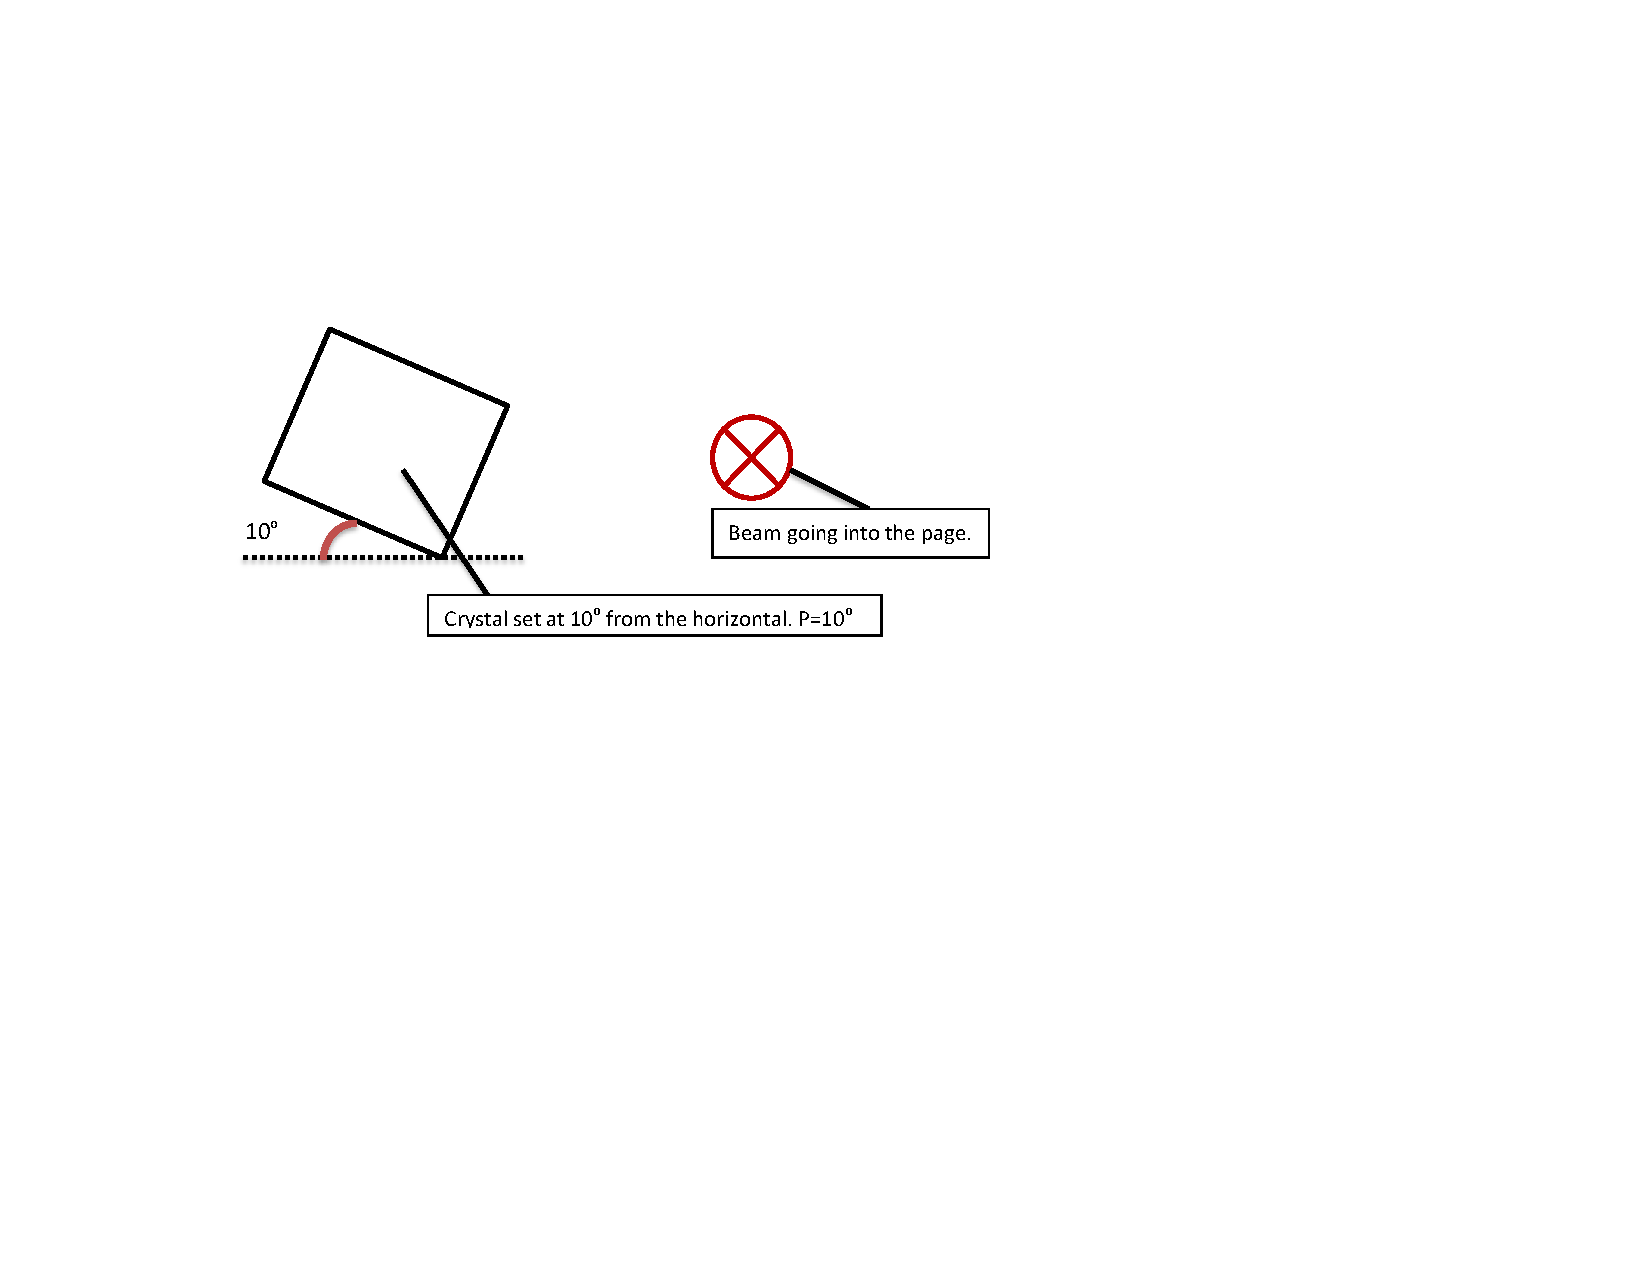
\includegraphics[width=0.5\textwidth]{Figs-for-Markus-from-JB-19-5-13-1.pdf}
\caption{Schematic of \Keyword{ANGLEP}. Figure courtesy of John Bremridge.}
\label{fig:angleP}
\end{figure}

\subsection{\Keyword{ANGLEL}}

\noindent \Keyword{ANGLEL \textit{F}}
sets the loop angle between the plane of the crystal loop and the goniometer axis. The angle is to be given in degrees, but without the degree symbol ($^\circ$). The default \textit{L} ('loop') angle is $0^\circ$.

The rotation angle to be applied to the angle of the crystal in the loop (right handed rotation about \textit{X} axis applied to all voxels, as shown in figure \ref{fig:angleL}).
\begin{figure}[h!]
\centering
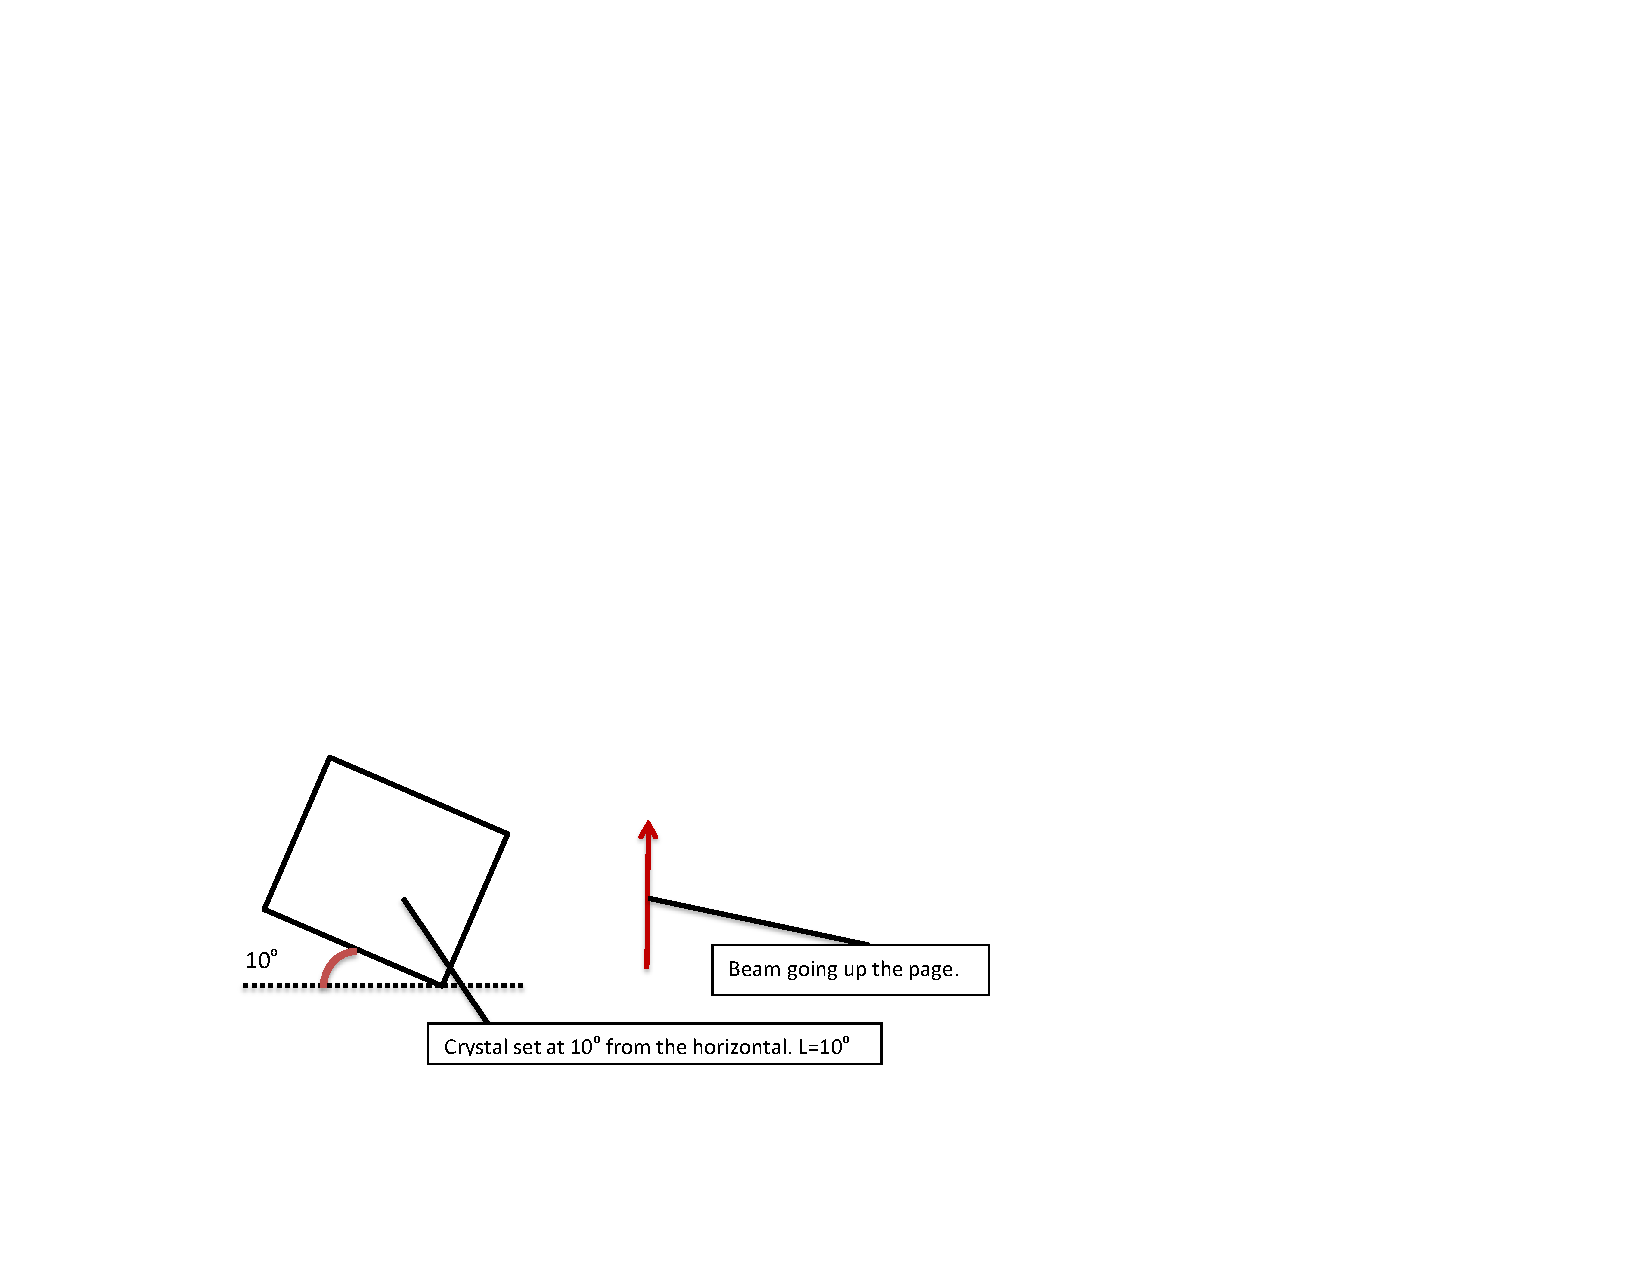
\includegraphics[width=0.5\textwidth]{Figs-for-Markus-from-JB-19-5-13-2.pdf}
\caption{Schematic of \Keyword{ANGLEL}. Figure courtesy of John Bremridge.}
\label{fig:angleL}
\end{figure}

\newpage

\subsection{\Keyword{CONTAINERMATERIALTYPE}}

\noindent \Keyword{CONTAINERMATERIALTYPE \textit{MATERIALTYPE}}
Specifies the material type of the container that encases the irradiated sample. This keyword should be used when the sample is encased within a container e.g. SAXS experiment where the sample is irradiated through a capillary. Currently three distinct container material type implementations exist:\SB

\noindent \Keyword{CONTAINERMATERIALTYPE NONE}
The sample is not encased inside any type of container hence there is no attenuation of the beam prior to making contact with the sample. This is the case with a standard X-ray crystallography experiment. This option is selected as the default if the \Keyword{CONTAINERMATERIALTYPE} is not defined.\SB

\noindent \Keyword{CONTAINERMATERIALTYPE MIXTURE}
Defines a container encasing the irradiated sample which is a mixture of elements, determined by the name of the mixture. If this option is used then the user must specify the material mixture (see section \hyperref[materialmixture]{\Keyword{MATERIALMIXTURE}}).\SB

\noindent \Keyword{CONTAINERMATERIALTYPE ELEMENTAL}
Defines a container encasing the irradiated sample in terms of its component elements. If this option is used then the user must specify the list of the material's component elements (see section \hyperref[materialelements]{\Keyword{MATERIALELEMENTS}}).\SB

\subsection{\Keyword{MATERIALMIXTURE}}
\label{materialmixture}
\noindent \Keyword{MATERIALMIXTURE \textit{MATERIAL}}
Specifies the material of the container that encases the irradiated sample by its mixture name. The exact input for \Keyword{\textit{MATERIAL}} is given in the URL of the corresponding material on the National Institute of Standards and Technology (NIST) \href{http://physics.nist.gov/PhysRefData/XrayMassCoef/tab4.html}{Table 4 webpage (click here)}. For example, if the material through which the sample is irradiated is pyrex glass then click on the \href{http://physics.nist.gov/PhysRefData/XrayMassCoef/ComTab/pyrex.html}{`Glass, Borosilicate ``Pyrex''' link} and the URL is:
\newline
\href{http://physics.nist.gov/PhysRefData/XrayMassCoef/ComTab/pyrex.html}{http://physics.nist.gov/PhysRefData/XrayMassCoef/ComTab/\textbf{pyrex}.html.}
\newline
The material name is given immediately before the ``.html'' and after the last forward slash ``/'', in this case the word is ``pyrex''. Hence to set the container material to pyrex glass the input would be \Keyword{MATERIALMIXTURE \textit{pyrex}}. Note that the input is case sensitive an internet connection is required for this option to work.

\subsection{\Keyword{MATERIALELEMENTS}}
\label{materialelements}
\noindent \Keyword{MATERIALELEMENTS \textit{El I} (\textit{El I} (\textit{El I} ..))}
Specifies the material of the container that encases the irradiated sample by a list of the component elements of the material. The mass attenuation coefficients for each element are downloaded from the National Institute of Standards and Technology (NIST) \href{http://physics.nist.gov/PhysRefData/XrayMassCoef/tab3.html}{Table 3 webpage (click here)}. For example, if the material through which the sample is irradiated is quartz, which has the formula SiO$_2$ then the input would be \Keyword{MATERIALMIXTURE \textit{Si 1 O 2}}. Note that an internet connection is required for this option to work.

\subsection{\Keyword{CONTAINERTHICKNESS}}

\noindent \Keyword{CONTAINERTHICKNESS \textit{F}}
Specifies the thickness of the container encasing the irradiated sample. The thickness should be given in $\mu$m.

\subsection{\Keyword{CONTAINERDENSITY}}

\noindent \Keyword{CONTAINERDENSITY \textit{F}}
Specifies the density of the container encasing the irradiated sample. The density should be given in grams/centimetre.


\newpage
\subsection{\Keyword{ABSCOEFCALC}}
\label{abscoefcalc}
This keyword specifies whether the program should use average absorption and attenuation coefficients, or whether it should calculate them from input crystal parameters.\SB

\noindent \Keyword{ABSCOEFCALC AVERAGE}

\noindent \Keyword{ABSCOEFCALC DUMMY}

These two commands are equivalent. Each will cause \RD to assume an absorption coefficient of 0.237 mm$^{-1}$ and an attenuation coefficient of 0.281 mm$^{-1}$. These values are representative of an average crystal at an incident X-ray beam energy of 12.4 keV (1\AA). Please see Section 3 in the main paper for more details. Crystal composition keywords will have no effect.\SB

\noindent \Keyword{ABSCOEFCALC RD}

\noindent \Keyword{ABSCOEFCALC RDV2}

\noindent \Keyword{ABSCOEFCALC RDV3}

These three commands are equivalent. \RD will call a previous version of RADDOSE to estimate absorption and attenuation coefficients.\SB

\noindent \Keyword{ABSCOEFCALC RD3D}

This command will use the current RADDOSE-3D code to calculate the absorption and attenuation coefficients using the crystal composition specified by the user. (NOTE: If the crystal composition is specified then the \Keyword{RD3D} keyword is preferred over the other \Keyword{ABSCOEFCALC} keywords, particularly if the crystal contains DNA or RNA molecules).

% XXXX  Removed from paper version
% The path to the locally installed legacy RADDOSE executable can be specified using the \Keyword{-p} command line option (see section ...).

The composition of the crystal has to be described using the keywords
 \hyperref[unitcell]{\Keyword{UNITCELL}},
 \hyperref[nummonomers]{\Keyword{NUMMONOMERS}},
 \hyperref[numresidues]{\Keyword{NUMRESIDUES}},
 \hyperref[numrna]{\Keyword{NUMRNA}},
 \hyperref[numdna]{\Keyword{NUMDNA}},
 \hyperref[proteinheavyatoms]{\Keyword{PROTEINHEAVYATOMS}},
 \hyperref[solventheavyconc]{\Keyword{SOLVENTHEAVYCONC}} and
 \hyperref[solventfraction]{\Keyword{SOLVENTFRACTION}}.
The use of these keywords is described in the sections \ref{RDv3Start}--\ref{RDv3End} below. Note that the \Keyword{SOLVENTFRACTION} keyword is now optional. If it's not given then RADDOSE-3D will calculate it.\SB

\noindent \Keyword{ABSCOEFCALC EXP}

This command should be used if the crystal composition from a Protein Data Bank (PDB) entry is to be used instead of a user specified crystal composition. The current RADDOSE-3D code is then used to calculate the absorption and attenuation coefficients using the crystal composition from the PDB entry. The PDB entry must be specified using the \hyperref[pdb]{\Keyword{PDB} keyword} (\hyperref[pdb]{section~\ref*{pdb}}).\SB

\noindent \Keyword{ABSCOEFCALC SEQUENCE}

This command should be used if the sample composition from a sequence file is to be used instead of a user specified crystal composition. The sequence file should be in \href{https://en.wikipedia.org/wiki/FASTA_format}{\textbf{FASTA}} file format. If this command is used then the composition of the crystal can be specified using the following keywords
\hyperref[unitcell]{\Keyword{UNITCELL}},
\hyperref[seqfile]{\Keyword{SEQFILE}},
\hyperref[nummonomers]{\Keyword{NUMMONOMERS}},
\hyperref[solventheavyconc]{\Keyword{SOLVENTHEAVYCONC}}
\SB

\noindent \Keyword{ABSCOEFCALC SAXS}

This command will use the current RADDOSE-3D code to calculate the absorption and attenuation coefficients using the sample composition specified by the user similarly to the keyword \Keyword{RD3D}. The major difference is that instead of supplying the number of monomers using the keyword \Keyword{NUMMONOMERS}, the user supplies the protein concentration used in the SAXS experiment using the keyword \Keyword{PROTEINCONC} (see section \hyperref[proteinconc]{\Keyword{PROTEINCONC}}).
\newline
Note that RADDOSE-3D treats the irradiated samples as stationary objects. Therefore if the SAXS solution is flowed through the capillary during the exposure then a suitable exposure time for the relevant volume will need to be taken into account.\SB


\noindent \Keyword{ABSCOEFCALC SAXSSEQ}

This command will use the current RADDOSE-3D code to calculate the absorption and attenuation coefficients using the sample composition specified by the user similarly to the keyword \Keyword{SAXS}. The major difference is that you no longer need to give the number of residues or the protein heavy atom composition. Instead the user needs to specify where the sequence file is located using the \Keyword{SEQFILE}.\SB


\noindent \Keyword{ABSCOEFCALC SMALLMOLE}

This command will use the current RADDOSE-3D code to calculate the absorption and attenuation coefficients using the crystal composition specified by the user, similarly to the keyword \Keyword{RD3D} above. However, this indicates that a small molecule experiment is present, and as such the user must instead specify the composition of the crystal using the keywords \Keyword{SMALLMOLEATOMS}, \Keyword{UNITCELL} and \Keyword{NUMMONOMERS} to explicitly define the entire contents of the small molecule unit cell (including solvent atoms). Note that in this current version, no additional solvent atoms can be specified with \Keyword{SOLVENTHEAVYCONC} keyword provided below. \SB


\noindent \Keyword{ABSCOEFCALC CIF}

This option is also provided for small molecule experiments. This command should be used if the crystal composition from a supplied CIF-format file is to be used instead of a user specified crystal composition. The current RADDOSE-3D code is then used to calculate the absorption and attenuation coefficients using the crystal composition from the CIF entry. A full file path to the CIF-format file must be specified using the additional \hyperref[cif]{\Keyword{CIF} keyword}  (\hyperref[cif]{section~\ref*{cif}}).


\subsection{\Keyword{PDB}}
\label{pdb}

\noindent \Keyword{PDB \textit{CODE}}

Where \Keyword{\textit{CODE}} is the four letter code of the PDB entry to be downloaded. From the PDB entry \RD will calculate
 \hyperref[unitcell]{\Keyword{UNITCELL}},
 \hyperref[nummonomers]{\Keyword{NUMMONOMERS}},
 \hyperref[numresidues]{\Keyword{NUMRESIDUES}},
 \hyperref[numrna]{\Keyword{NUMRNA}},
 \hyperref[numdna]{\Keyword{NUMDNA}},
 \hyperref[proteinheavyatoms]{\Keyword{PROTEINHEAVYATOMS}} and
 \hyperref[solventfraction]{\Keyword{SOLVENTFRACTION}}, and hence these keywords are not needed.
It will NOT calculate \hyperref[solventheavyconc]{\Keyword{SOLVENTHEAVYCONC}} so if there are any heavy atoms in the solvent then they will have to be specified. Note that an internet connection is required for this option to work. \SB

\noindent \Keyword{PDB \textit{FILENAME}}

Where \Keyword{\textit{FILENAME}} specifies the location of the PDB file for the chosen sample. 
Only sequence files in the \href{https://en.wikipedia.org/wiki/Protein_Data_Bank_(file_format)}{\textbf{PDB}} format can be read. \SB


\subsection{\Keyword{SEQFILE}}
\label{seqfile}

\Keyword{SEQFILE \textit{FILENAME}} specifies the location of the file that contains the sequence of the chosen sample.
Only sequence files in the \href{https://en.wikipedia.org/wiki/FASTA_format}{\textbf{FASTA}} format can be read. \SB

\subsection{\Keyword{CIF}}
\label{cif}

\Keyword{CIF \textit{FILENAME}} specifies the location of the file that contains the sequence of the chosen sample. This is exclusively for small molecule experiments and only files in the \href{https://en.wikipedia.org/wiki/Crystallographic_Information_File}{\textbf{CIF}} format can be read. \SB

\subsection{\Keyword{UNITCELL}}
\label{RDv3Start}
\label{unitcell}
\RDLegacyKeyword

\noindent \Keyword{UNITCELL \textit{A B C}}

\noindent \Keyword{UNITCELL \textit{A B C $\alpha$ $\beta$ $\gamma$}}

Dimensions and angles of the unit cell a, b, c, $\alpha$, $\beta$, $\gamma$

The first three numbers specify the unit cell size in Angstroms. The second three numbers optionally specify the unit cell angles alpha, beta and gamma.

The (optional) angles are to be given in degrees, but without the degree symbol ($^\circ$). If no angles are specified \RD assumes default angles of $90^\circ$.

\subsection{\Keyword{NUMMONOMERS}}
\label{nummonomers}
\RDLegacyKeyword

\noindent \Keyword{NUMMONOMERS \textit{I}}
specifies the number of monomers in the unit cell. Only integer numbers \textit{I} should be used. This number should not be confused with the number of monomers in the asymmetric unit.


\subsection{\Keyword{NUMRESIDUES}}
\label{numresidues}
\RDLegacyKeyword

\noindent \Keyword{NUMRESIDUES \textit{I}}
specifies the number of amino acid residues per monomer. Only integer numbers \textit{I} should be used. Using this keyword the number and types of atoms are calculated according to the formula
\[ \mbox{amino acid} = 5 C + 1.35 N + 1.5 O + 8 H \]
Sulfur atoms, e.g. from CYS and MET residues, should be added explicitly with \hyperref[proteinheavyatoms]{the \Keyword{PROTEINHEAVYATOMS} keyword}.

The default value for \textit{I} is 0.


\subsection{\Keyword{NUMRNA}}
\label{numrna}
\RDLegacyKeyword

\noindent \Keyword{NUMRNA \textit{I}}
specifies the number of RNA nucleotides per monomer. Only integer numbers \textit{I} should be used. Using this keyword the number and types of atoms are calculated assuming an average nucleotide content defined as
\[ \mbox{mean nucleotide} = 11.25H + 9.5C + 3.75N + 7O + 1P \]
If a more accurate estimate is required, individual atoms may be entered explicitly with \hyperref[proteinheavyatoms]{the \Keyword{PROTEINHEAVYATOMS} keyword}.

The default value for \textit{I} is 0.


\subsection{\Keyword{NUMDNA}}
\label{numdna}
\RDLegacyKeyword

\noindent \Keyword{NUMDNA \textit{I}}

specifies the number of DNA deoxynucleotides per monomer. Only integer numbers \textit{I} should be used. Using this keyword the number and types of atoms are calculated assuming an average deoxynucleotide content defined as
\[ \mbox{mean nucleotide} = 11.75H + 9.75C + 4N + 6O + 1P \]
If a more accurate estimate is required, individual atoms may be entered explicitly with \hyperref[proteinheavyatoms]{the \Keyword{PROTEINHEAVYATOMS} keyword}.

The default value for \textit{I} is 0.


\subsection{\Keyword{PROTEINHEAVYATOMS}}
\label{proteinheavyatoms}
\RDLegacyKeyword

\noindent \Keyword{PROTEINHEAVYATOMS \textit{El I} (\textit{El I} (\textit{El I} ..))}
defines a list of atoms to add to the protein part of the absorption. Each species is defined by a two character string \Keyword{\textit{El}} for the elemental symbol, and an integer number \Keyword{\textit{I}} of atoms of that species per monomer.

The command \Keyword{PROTEINHEAVYATOMS S 10 Se 2} would add 10 sulfur and 2 selenium atoms per monomer.


\subsection{\Keyword{SOLVENTHEAVYCONC}}
\label{solventheavyconc}
\RDLegacyKeyword

\noindent \Keyword{SOLVENTHEAVYCONC \textit{El I} (\textit{El I} (\textit{El I} ..))}
defines the concentration of elements (not including water) in the solvent in millimoles per litre. Oxygen and lighter elements should not be specified.

The command \Keyword{SOLVENTHEAVYCONC Na 1000 Cl 1000} specifies 1M sodium chloride in the solvent.


\subsection{\Keyword{SOLVENTFRACTION}}
\label{solventfraction}
\RDLegacyKeyword

\noindent \Keyword{SOLVENTFRACTION \textit{F}}

The fraction of the unit cell that is occupied by solvent. If not given explicitly, this value is estimated from \hyperref[numresidues]{\Keyword{NUMRESIDUES}}, \hyperref[numrna]{\Keyword{NUMRNA}} and \hyperref[numdna]{\Keyword{NUMDNA}} using 1.35 g/ml for protein, and 1.35 g/ml for DNA and 1.3 g/ml for RNA.

% \hyperref[proteinheavyatoms]{the \Keyword{PROTEINHEAVYATOMS} keyword}.

\subsection{\Keyword{PROTEINCONC}}
\label{proteinconc}
This keyword only has an effect when the absorption and attenuation coefficients are estimated using the keyword \Keyword{SAXS} \hyperref[abscoefcalc]{section \ref*{abscoefcalc}\SB}

\noindent \Keyword{PROTEINCONC \textit{F}}

The protein concentration used in the SAXS experiment in grams per litre.


\subsection{\Keyword{SMALLMOLEATOMS}}
\label{amallmoleatoms}
This keyword only has an effect when the absorption and attenuation coefficients are estimated using the keyword \Keyword{SMALLMOLE} \hyperref[abscoefcalc]{section \ref*{abscoefcalc}\SB} and is only to be used for small molecule experiments

\noindent \Keyword{SMALLMOLEATOMS \textit{El I} (\textit{El I} (\textit{El I} ..))}
defines a list of atoms to explicitly define the full contents of the unit cell. Each species is defined by a two character string \Keyword{\textit{El}} for the elemental symbol, and an integer number \Keyword{\textit{I}} of atoms of that species per `monomer' in the unit cell (note that if the  \Keyword{NUMMONOMERS} keyword is omitted from the input file, then 1 monomer is assumed per unit cell).

The command \Keyword{SMALLMOLEATOMS C 18 H 15 Bi 8} would add 18 carbon 15 hydrogen and 8 bismuth atoms per `monomer' in the unit cell.

\subsection{\Keyword{CALCULATEPEESCAPE}}
\label{calculatepeescape}

\noindent \Keyword{CALCULATEPEESCAPE \textit{BOOLEAN}}
Whether or not to include an explicit 3D model for photoelectron escape from the crystal volume. Set to \Keyword{\textit{TRUE}} to include or \Keyword{\textit{FALSE}} otherwise (defaults to \Keyword{\textit{FALSE}} if not set). 

\subsection{\Keyword{CALCULATEFLESCAPE}}
\label{calculateflescape}

\noindent \Keyword{CALCULATEFLESCAPE \textit{BOOLEAN}}
Whether or not to include an explicit 3D model for fluorescent X-ray escape from the crystal volume. Set to \Keyword{\textit{TRUE}} to include or \Keyword{\textit{FALSE}} otherwise (defaults to \Keyword{\textit{FALSE}} if not set).

\subsection{\Keyword{CALCSURROUNDING}}
\label{calcsurrounding}

\noindent \Keyword{CALCSURROUNDING \textit{BOOLEAN}}
Whether or not to include photoelectron entry from the surrounding material into the crystal volume. Set to \Keyword{\textit{TRUE}} to include or \Keyword{\textit{FALSE}} otherwise (defaults to \Keyword{\textit{FALSE}} if not set).
Note that \Keyword{CALCULATEPEESCAPE} must be set to \Keyword{\textit{TRUE}} for this option to be used.

\subsection{\Keyword{OILBASED}}
\label{oilbased}

\noindent \Keyword{OILBASED \textit{BOOLEAN}}
Whether or not the surrounding is oil based. Set to \Keyword{\textit{TRUE}} to indicate oil based or \Keyword{\textit{FALSE}} otherwise (defaults to \Keyword{\textit{FALSE}} if not set).

\subsection{\Keyword{SURROUNDINGHEAVYCONC}}
\label{surroundingheavyconc}

\noindent \Keyword{SURROUNDINGHEAVYCONC \textit{El I} (\textit{El I} (\textit{El I} ..))}
defines the concentration of elements (not including water) in the solvent in millimoles per litre. Oxygen and lighter elements should not be specified.

The command \Keyword{SOLVENTHEAVYCONC Na 1000 Cl 1000} specifies 1M sodium chloride in the surrounding.

Note if \Keyword{OILBASED} is set to \Keyword{\textit{TRUE}}, all elements in the surrounding must be specified.

\label{RDv3End}


\section{\Class{Beam} block}

A \Class{Beam} block must begin with the keyword \Keyword{BEAM}.
At least the \hyperref[beamtype]{\Keyword{TYPE}} must be specified.
Depending on the chosen \hyperref[beamtype]{\Keyword{TYPE}}, further declarations may be required.


\subsection{\Keyword{TYPE}}
\label{beamtype}

With the keyword \Keyword{TYPE}, the underlying beam implementation is chosen.
Currently three distinct beam implementations exist:\SB

\noindent \Keyword{TYPE TOPHAT} defines a beam with uniform flux.\SB

\noindent \Keyword{TYPE GAUSSIAN} defines a beam with a 2-dimensional Gaussian flux profile. The full-width half-maximum must be specified with \hyperref[beamfwhm]{the \Keyword{FWHM} keyword} (see \hyperref[beamfwhm]{section~\ref*{beamfwhm}}).\SB

\noindent \Keyword{TYPE EXPERIMENTALPGM} defines an arbitrary beam profile as defined in a given portable graymap file (.pgm) specified with \hyperref[file]{the \Keyword{FILE} keyword} (see \hyperref[file]{section~\ref*{file}}). The pixel size of the image file also has to be specified with \hyperref[pixelsize]{the \Keyword{PIXELSIZE} keyword} (see \hyperref[pixelsize]{section~\ref*{pixelsize}}).\SB


\subsection{\Keyword{FLUX}}
\label{flux}

\noindent \Keyword{FLUX \textit{F}} specifies the total beam flux in photons per second. The flux parameter \textit{F} can be specified in scientific notation (e.g. \Keyword{1.3e12}).


\subsection{\Keyword{FWHM}}

\label{beamfwhm}
\noindent \Keyword{FWHM \textit{X Y}}

The FWHM of the beam (vertical), (horizontal). Not needed if a Top-Hat beam is used.
This defines the \textit{X} and \textit{Y} FWHM of the beam respectively in the RADDOSE coordinate system.


\subsection{\Keyword{ENERGY}}

\noindent \Keyword{ENERGY \textit{F}}

\noindent \Keyword{ENERGY \textit{F} KEV}

specifies the incident photon energy in keV. The optional keyword \Keyword{KEV} can be appended for human readability of the input file.

\subsection{\Keyword{FILE}}
\label{file}

\noindent \Keyword{FILE \textit{SOMEPGMFILE.PGM}}

specifies the location of the .pgm file that describes the beam profile. NOTE: the .pgm file should be in ASCII format. The pixel size of the image file also has to be specified with \hyperref[pixelsize]{the \Keyword{PIXELSIZE} keyword} (see \hyperref[pixelsize]{section~\ref*{pixelsize}}).\SB

\subsection{\Keyword{PIXELSIZE}}
\label{pixelsize}

\noindent \Keyword{PIXELSIZE \textit{X Y}}.

\Keyword{\textit{X}} and \Keyword{\textit{Y}} specify the horizontal and vertical size of the pixels in micrometers in the .pgm file respectively.

\subsection{\Keyword{COLLIMATION}}

\noindent \Keyword{COLLIMATION RECTANGULAR \textit{X Y}}

specifies the horizontal and vertical collimation of the beam.
Delimits where the beam has non-zero intensity.
This is defined by the slits.
For an uncollimated Gaussian beam, set to $\approx 3 \times$ FWHM. \SB


\noindent \Keyword{COLLIMATION CIRCULAR \textit{X Y}}

specifies the horizontal and vertical collimation of a circular or elliptical beam.
Delimits where the beam has non-zero intensity.
This is defined by the slits.

%\noindent \Keyword{COLLIMATION HORIZONTAL \textit{F}}
%(not supported!)
%
%\noindent \Keyword{COLLIMATION VERTICAL \textit{F}}
%(not supported!)

\section{\Class{Wedge} block}

A \Class{Wedge} block must begin with the keyword \Keyword{WEDGE}.

\Keyword{WEDGE \textit{A B}}

\textit{A} and \textit{B} define the start and end angle of the rotation in degrees ($^\circ$). At $0^\circ$ the front face of the crystal (\textit{X-Y} plane) is normal to the beam. Rotation is right handed about the \textit{Y} axis, as shown in figure \ref{fig:anglePhi}).
\begin{figure}[h!]
\centering
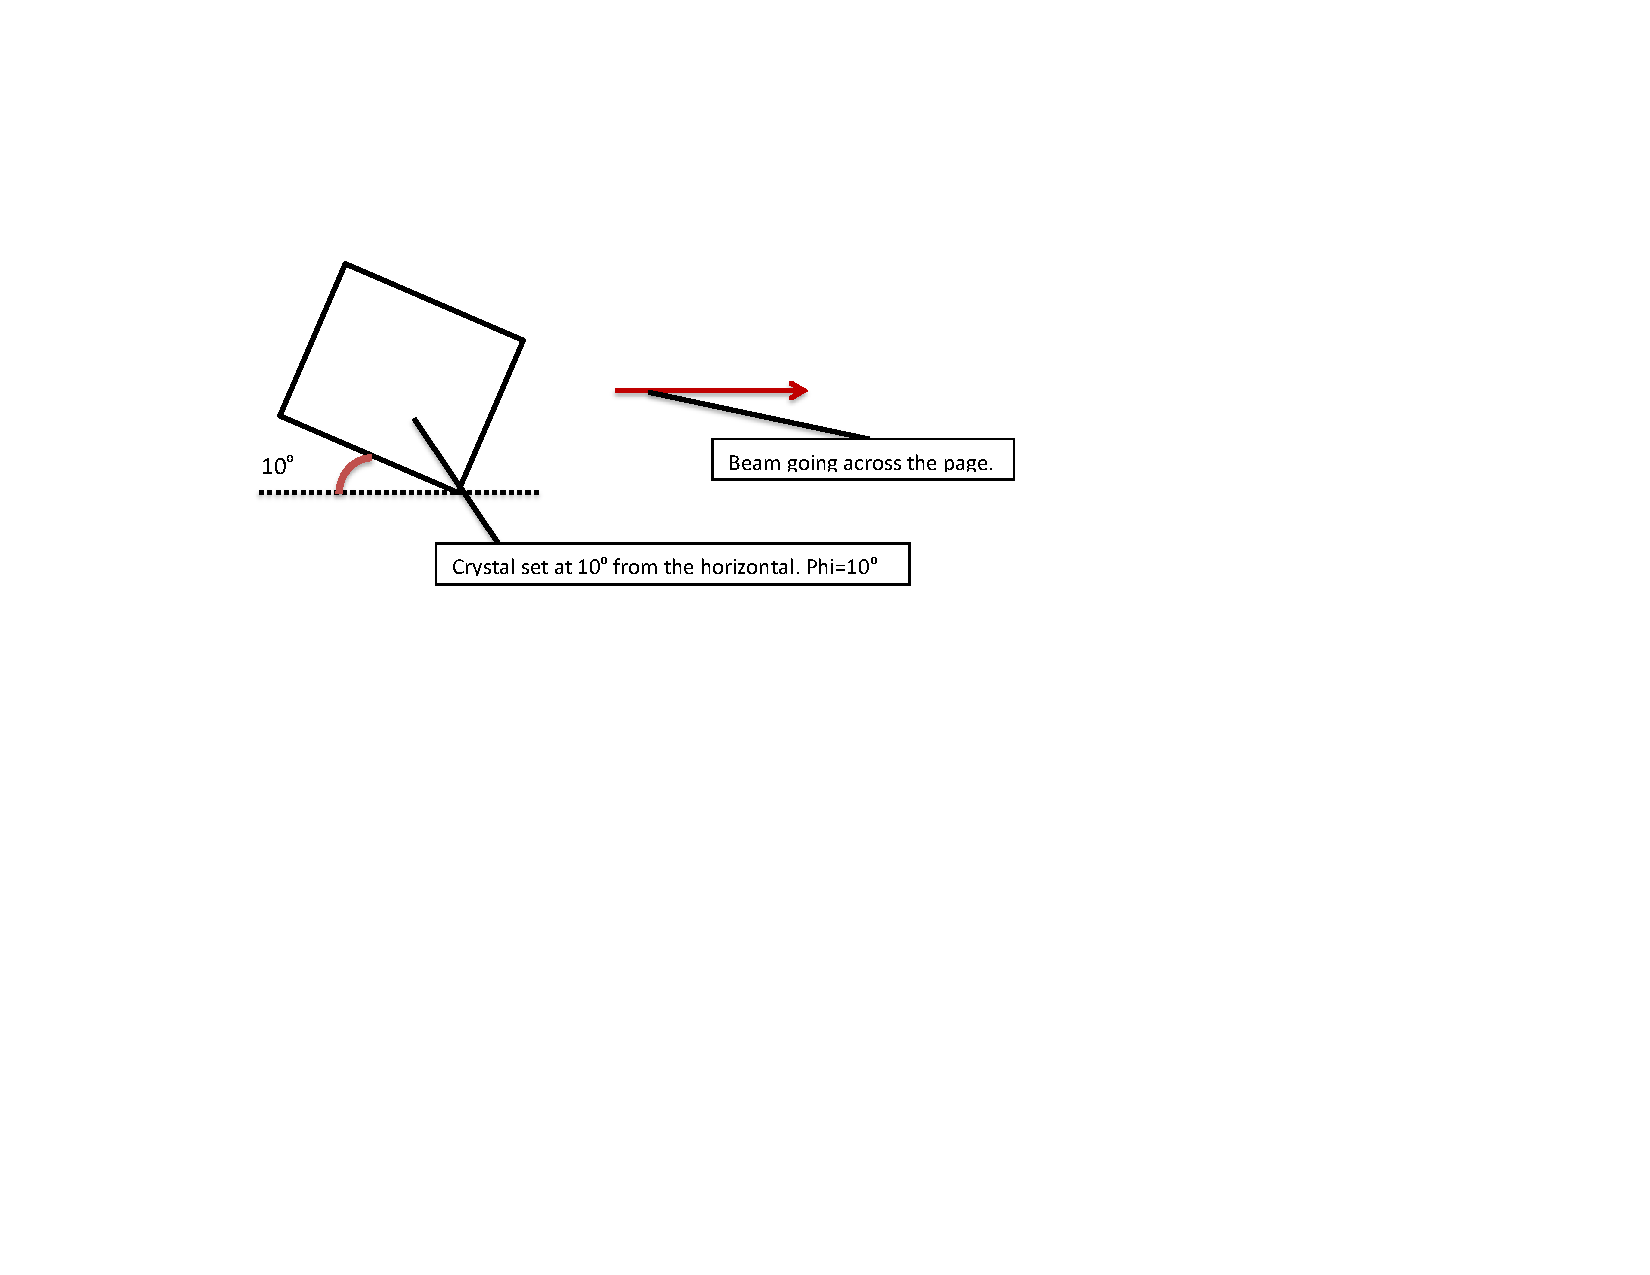
\includegraphics[width=0.5\textwidth]{Figs-for-Markus-from-JB-19-5-13-3.pdf}
\caption{Schematic of angles for \Keyword{WEDGE}. Figure courtesy of John Bremridge.}
\label{fig:anglePhi}
\end{figure}

\subsection{\Keyword{EXPOSURETIME}}

\noindent \Keyword{EXPOSURETIME \textit{F}}

specifies the total exposure time for this wedge in seconds.



\subsection{\Keyword{ANGULARRESOLUTION}}

\noindent \Keyword{ANGULARRESOLUTION \textit{F}}

specifies the angular step size used for wedge iterations in degrees ($^\circ$). Defaults to $2^\circ$.
\newline
Note: If very small wedges are being used e.g. $<5^{\circ}$ then the angular resolution should be decreased.



\subsection{\Keyword{STARTOFFSET}}

\noindent \Keyword{STARTOFFSET \textit{X Y Z}}

offset translation in \hbox{\textmu}m applied to the crystal relative to the origin (defined as the intersection of the beam and the aligned goniometer axis) for the starting position of the wedge. Defaults to 0 0 0.



\subsection{\Keyword{TRANSLATEPERDEGREE}}

\noindent \Keyword{TRANSLATEPERDEGREE \textit{X Y Z}}

translation of the goniometer during exposure in \hbox{\textmu}m$/^{\circ}$ for helical scanning, leading to improvements in dose distribution. Defaults to 0 0 0.



\subsection{\Keyword{ROTAXBEAMOFFSET}}

\noindent \Keyword{ROTAXBEAMOFFSET \textit{F}}

the offset in \hbox{\textmu}m along \textit{X} (vertical in most set-ups) between the beam axis and the rotation axis. Used to create 'offset' scanning for improvements in dose distribution. Defaults to 0 \hbox{\textmu}m.

\end{document}
